\documentclass[debug,journal]{rmaa}

% \makeatletter
% \renewcommand{\rmaa@VolumeStyle}[1]{#1}
% \renewcommand{\rmaa@JournalNameStyle}[1]{#1}
% \makeatother

%%%
%%% Load any optional packages you need here with \usepackage
%%% 

% This allows compact, in-paragraph, and as-paragraph  versions of the
% standard itemize and enumerate environments. 
\usepackage{paralist}

% These are used in one of the graphics examples
\usepackage{psfrag,color}

% Allow accented characters to be entered directly
\usepackage[latin1]{inputenc}
%%%
%%% Define any personal macros here
%%% 

% These are some I use in typesetting example code
\newcommand{\bs}{\textbackslash}
\newcommand{\CS}[1]{\texttt{\textbackslash #1}}
\newenvironment{Example}
{\begin{list}{}{\setlength{\leftmargin}{10pt}\setlength{\rightmargin}{10pt}}%
  \item[]\itshape}
  {\end{list}}

% Needed for landscape tables
\usepackage{pdflscape}

% \newcommand\orcidicon{
\includegraphics[height=1.8ex]{ORCIDiD_iconvector}}
% \newcommand\orcidiconbig{
\includegraphics[height=2ex]{ORCIDiD_iconvector}}
% %\newcommand\href[2]{#2}
% \newcommand\ORCIDiD[1]{\href{https://orcid.org/#1}{\,\orcidicon}}
% \newcommand\ORCIDiDfull[1]{\href{https://orcid.org/#1}{\orcidiconbig}\,\url{https://orcid.org/#1}}


%%%
%%% Article preamble commands (title, authors, abstract, etc.) 
%%% None of these produce any output themselves, they just set things 
%%% up for \maketitle
%%%

% Please use mixed case here, since this title gets propagated onto
% the web page, ADS entry, etc. 
\title{A Demonstration Document for the RevMexAA Main Journal} 

% For the conference proceedings, the author affiliations should be
% subscripted, using \altaffil and/or \altaffilmark + \altaffiltext
% Note that \altaffilmark goes after a comma and that `and' is spelt
% out.
\author{
  W. J. Henney\ORCIDiD{0000-0001-6208-9109},\altaffilmark{1} 
  A. Collaborator,\altaffilmark{2}
  and L. Author\altaffilmark{2,3,4}}

% Note that \altaffil, \altaffilmark go inside the scope of the
% \author{...} command but \altaffiltext is outside it. 
\altaffiltext{1}{Instituto de Radioastronom\'\i{}a y Astrof\'\i{}sica,
  UNAM, Morelia, M\'exico.}

\altaffiltext{2}{Instituto de Astronom\'\i{}a, UNAM, CDMX, M\'exico.}

\altaffiltext{3}{Please note that affiliations end in periods.  In the
  main journal, full postal addresses are given at the end of the
  paper, with only abbreviated versions appearing here.}

% Authors for running headers - surnames only, et al. if more than 3. 
\shortauthor{Henney, Collaborator, \& Author}
% Title for running header
\shorttitle{RevMexAA Main Journal Demo Document}


% \newaffiliation {IRyA} {Instituto de Radioastronom\'\i{}a y
%   Astrof\'\i{}sica, UNAM, M\'exico} {Instituto de Radioastronom\'\i{}a
%   y Astrof\'\i{}sica, Universidad Nacional Aut\'onoma de M\'exico,
%   Apartado Postal 3--72, 58090 Morelia, Michoac\'an, M\'exico}

% \authorinfo{
%   \authorORCID
%   \authorAFFIL{IRyA}
% }

% Define macros for each full address to save repetition
\newcommand\IRyA{Instituto de Radioastronom\'\i{}a y
  Astrof\'\i{}sica, Universidad Nacional Aut\'onoma de M\'exico,
  Apartado Postal 3--72, 58090 Morelia, Michoac\'an, M\'exico}
\newcommand\IAUNAM{Instituto de Astronom\'\i{}a, Universidad Nacional
  Aut\'onoma de M\'exico, Apartado Postal 70-264, M\'exico, CDMX,
  C.P. 04510}

% Full postal addresses (in alphabetical surname order!)
% plus email addresses in parentheses. 
\fulladdresses{
% Formatted in list environment, so each group is an \item
\item Last Author\ORCIDiD{0000-0001-6208-9109} and Another
  Collaborator\ORCIDiD{0000-0001-6208-9109}: \IAUNAM{} (la,
  ac@astro.unam.mx).
% Note final period.
\item William J. Henney\ORCIDiD{0000-0001-6208-9109}: \IRyA{}
  (w.henney@irya.unam.mx). }


% List of authors used to construct table of contents
\listofauthors{W. J. Henney, A. Collaborator, \& L. Author}
% Each author in Surname, Initials format, used in generating Author
% Index entries.
\indexauthor{Henney, W. J.}
\indexauthor{Collaborator, A.}
\indexauthor{Author, L.}


% Give data for ADS affiliations
\AuthorADS{Henney, W. J.}{
  \Affil{\IRyA} \ORCIDiD{0000-0001-6208-9109} \Email{w.henney@irya.unam.mx}
}
\AuthorADS{Collaborator, A.}{
  \Affil{\IAUNAM} \ORCIDiD{0000-0000-0000-0000} \Email{ac@astro.unam.mx}
}
\AuthorADS{Author, L.}{
  \Affil{\IAUNAM} \ORCIDiD{0000-0000-0000-0000} \Email{la@astro.unam.mx}
}


% English abstract
\abstract{This document (\texttt{rm-journal-example.tex}---last
  updated 2019 November 12) gives a brief tutorial in the use of
  version 3 of the \texttt{rmaa} \LaTeX{} macros and can also serve as
  a template for the preparation of papers to be published in the main
  journal. More details can be found in the user guide
  (\texttt{authorguide.pdf}).  It is assumed that you are already
  familiar with the rudiments of \LaTeX{}. In case you are not, some
  suitable references are given in \texttt{authorguide.pdf}.}

% Spanish abstract - leave blank and it will be translated by the
% editors. 
\resumen{Este documento (\texttt{rm-journal-example.tex}---�ltima
  actualizaci�n 12 de noviembre del 2019) proporciona un tutorial
  breve en el uso de la versi�n 3 de los macros de \LaTeX{}
  \texttt{rmaa} y adem�s puede servir c�mo modelo para la preparaci�n
  de los art�culos que se publicar�n en la revista principal. Se puede
  encontrar m�s detalles en la gu�a del usuario
  (\texttt{authorguide.pdf}). Se supone que usted es ya familiar con
  los rudimentos del \LaTeX{}. En el caso contrario, se dan
  algunas referencias convenientes en el \texttt{authorguide.pdf}.}


% Keywords must be from the standard list and in alphabetical order. 
\addkeyword{H~II regions}
\addkeyword{ISM: Jets and outflows}
\addkeyword{Stars: Pre-main sequence}
\addkeyword{Stars: Mass loss}

%\DOI{2019.55.02.21}
%%%
%%% Beginning of document proper
%%%
\begin{document}
% Typeset article header
\maketitle


\section{General}
\label{sec:intro}

Articles to be considered for publication in the main journal should
be prepared in the ``manuscript'' style, which is now the default when
no explicit options are given to the \CS{documentclass} command. The
reason for this is to allow authors to concentrate on the content of
their paper, rather than the details of the typesetting. This style
also has ample margins to allow a comfortable number of words per line
and to leave room for marginal notes.

Please use standard \LaTeX{} sectioning commands to subdivide your
document. You should use mixed case for the section titles, although
in the current style this only really matters at the level of
\CS{subsection} and below.

It is preferable to use the \CS{label}/\CS{ref} mechanism for
cross-references in order to
\begin{inparaenum}[(1)]
\item minimise the chance of errors, and 
\item allow automatic hyperlinks in PDF output (finally implemented in
  version 3.27).
\end{inparaenum}
Note that this sometimes requires \LaTeX{} to be run twice inorder to
resolve all of the references.

The style that should be used for cross-references is, for example,
Figure~\ref{fig:crop}, Table~\ref{tab:ion_ab},
equation~(\ref{eq:one}), and \S~\ref{sec:EPS}, where the section
symbol ``\S'' is produced by the \LaTeX\ command ``\CS{S}''.

General typographic best practices are discussed in
\S~\ref{sec:errors}, while following sections discuss how to format
include figure (\S~\ref{sec:EPS}), tables (\S~\ref{sec:how-do-tables})
and citations (\S~\ref{sec:refs}).

\section{Best Practices for Typesetting your Paper}
\label{sec:errors}

Usually, the right way of doing things is no more difficult
than the wrong way, once you have learned it.   

\subsection{Special Commands Inherited from AAS Macros}
\label{sec:command}

The \texttt{rmaa} macros implement all the ``astronomical'' commands
defined in the AAS\TeX{} macros. Please try to use these since it
helps ensure consistency of appearance and usage between papers. In
many cases I have tried to improve on the AAS\TeX{}
implementations. Commonly used examples are 
\begin{enumerate}
\item The \CS{ion} command: \ion{H}{ii}, \ion{Fe}{26}, etc. This can
  be happily used inside or outside math mode and inside figure
  captions. The ion stage can be specified as an arabic or roman
  numeral: \verb+\ion{H}{2}+, \verb+\ion{H}{ii}+, and
  \verb+\ion{H}{II}+ will all produce the same output. One caveat:
  \CS{ion} cannot be used inside the \CS{addkeyword} command---just
  use \verb+H~II+ there if necessary.
\item The \CS{arcsec}, \CS{arcmin} and \CS{arcdeg} commands, together
  with their ``fractional'' relatives, \CS{farcs}, etc. These are used
  in the following way: 
  \begin{Example}
    \verb|at declination|\\
    \verb|15\arcdeg\,33\arcmin\,22\farcs{}2|\\[\smallskipamount]
    \dots at declination $15\arcdeg\,33\arcmin\,22\farcs{}2$ \dots
  \end{Example}
  Again, they can be used inside or outside math mode. 
\end{enumerate}


\subsection{Math Symbols and Equations}
\label{sec:math}

Symbols for physical quantities should usually be italic: velocity,
$v$, density, $N$, etc. However, multi-letter symbols generally look
better in roman: FWHM, EM, etc. Subscripts should be in roman (coded
using \CS{mathrm}) unless they are themselves variables:
$N_\mathrm{e}$, $T_\mathrm{eff}$, but $\sum_i a_i$. Physical units
should in roman, with thin spaces: $10\,\mathrm{K}$, $1.2\times
10^{-12} \,\mathrm{erg\,cm^{-2}\,s^{-1}}$, etc. Things generally come
out best if you place an entire expression within a single pair of
\$'s and then make judicious use of \CS{mathrm}. For example
\begin{Example}
  $ \mathrm{FWHM} = \int N_\mathrm{e} N_\mathrm{i} \, dz $ 
\end{Example}
Remember that the ``minus sign'' only exists inside math mode: minus
two is $-2$, not~-2, nor \hbox{even --2!} Also, remember that spacing inside
math mode is designed for equations, not words, so you shouldn't use
\$'s just to get italic text. Compare $effective$ and
\textit{effective}. 

The \CS{frac} command (and its \TeX{} relative \CS{over}) are best
only used in displayed equations. Something like 
\begin{equation}
  \label{eq:one}
  x = \frac { a + b } { c } 
\end{equation}
looks fine, whereas $x = \frac { a + b } { c }$ is somewhat cramped.
Better rewritten as $x = (a + b) / c $. 

\paragraph{How to define a macro that can be used inside or outside
  math mode.} Use the \CS{ensuremath} command. For instance: 
\begin{verbatim}
\newcommand{\fluxunits}{%
   \ensuremath{\mathrm{%
      erg\,s^{-1}\,cm^{-2}}}}
\end{verbatim}
Then you can write either \verb+15.1\,\fluxunits+ or
\verb+$2.3\times+ \verb+10^{-11} \,+ \verb+\fluxunits$+


\subsection{Spacing After Periods}
\label{sec:space}

\TeX{}/\LaTeX{} distinguishes between inter-word spaces and
inter-sentence spaces. The latter are slightly wider and considerably
more ``stretchy'' than the former. A period that follows a lower-case
letter is assumed to end a sentence, while one that follows an
upper-case letter is not.  This heuristic produces correct results
99\% of the time, but there are two cases where you need to give a
helping hand by using the \verb+\@+ command, which causes \LaTeX{} to
``forget'' what was just before it. 


\paragraph{Lower case abbreviations ending in periods.} The only common
example is ``et~al.\@'', which should always be coded as, for example,
\begin{Example}
  \verb+Henney et~al.\@ (2002).+
\end{Example} 
Other examples, such as ``e.g.\@'' and ``i.e.\@'' should normally be
followed by a comma, so do not present this problem. The only other
example I have encountered is ``cf.\@'' but this should be followed by
a tie since we don't want a linebreak between it and the following
word:
\begin{Example}
  \verb+(cf.~Jones 1990)+
\end{Example}


\paragraph{Sentences that end in a capital letter.} These are more common
than you might think and should be coded as in the following examples. 
\begin{Example}
  \verb+provided by NASA\@. Next sentence+\\
  \makebox[1.05\width][s]{\dots provided by NASA\@. Next sentence \dots}\\[0.5\baselineskip]
  \verb+a width of 1.5\,\AA\@. Next sentence+\\
  \makebox[1.05\width][s]{\dots a width of 1.5\,\AA\@. Next sentence \dots}
\end{Example}
Note that ``\AA'' is considered by \LaTeX{} to be a capital letter, as
in the second example. 



\subsection{Spacing in/after macros}
\label{sec:macrospace}
It is never a good idea to include explicit space at the end of a
definition of a user macro. Examples such as the following should be
avoided:
\begin{Example}
  \verb+\newcommand{\kms}{km\,s$^{-1}$\ }+ \hfill\textbf{Wrong!}
\end{Example}
This will make the spacing come out right when you write
\begin{Example}
  \newcommand{\kms}{km\,s$^{-1}$\ }
  \verb+a speed of 5000~\kms is quite fast+\\
  a speed of 5000\,\kms is quite fast
\end{Example}
but it won't work if the macro is followed by a punctuation mark, such
as 
\begin{Example}
  \newcommand{\kms}{km\,s$^{-1}$\ }
  \verb+with values 5~\kms, 10~\kms, and+\\
  with values 5\,\kms, 10\,\kms, and \dots
\end{Example}

The right way\footnote{Of course, an even better way would be to use
  \CS{ensuremath}, as described above in \S~\ref{sec:math}} to go
about this is to define the macro without any following space:
\begin{Example}
  \verb+\newcommand{\kms}{km\,s$^{-1}$}+ \hfill\textbf{Right!}
\end{Example}
Then, whenever you use the macro \emph{always} follow it with an empty
pair of braces, i.e., \verb+\kms{}+. That way the spacing will come
out right in all circumstances. 


\subsection{Avoid Excessive Fiddling With the Layout }
\label{sec:fiddling}

The \texttt{rmaa} macros include various commands for final tweaking
of a paper, such as \CS{adjustfinalcols}, \CS{RescaleTitleLengths},
etc.  There is little value in using these for a submitted manuscript.
However, authors may want to us them to fine-tune the appearance of a
preprint.  

\subsection{Other Minor Points}
\label{sec:little}

By tradition, satellites should be in italic: \textit{HST},
\textit{ISO}, etc. Don't ask me why. 

Compound adjectives are generally hyphenated, whereas the
corresponding noun is not. E.g., ``mass-loading rate'' but ``in the
absence of mass loading''. However, you shouldn't hyphenate a number
(written as digits) and a unit. E.g., ``using a 4~m telescope'', ``we
observed 15~GHz emission''. 

A range of numbers is indicated by an ``en-dash'' (--), coded as
\verb+--+, as in ``in the range 4000--6000\,\AA''. An ``em dash''
(---), coded as \verb+---+ is used for punctuation. For example: 
\begin{Example}
  We also stress that our observations---at a single
  wavelength---cannot confirm the thermal nature of the emission.
\end{Example}
There should be  no space around the ``---''. 

Numbers larger than 9999 should have a comma. E.g., 10,000\,K but
9000\,K\@.

\section{Including Figures}
\label{sec:EPS}

\begin{figure}[!t]
  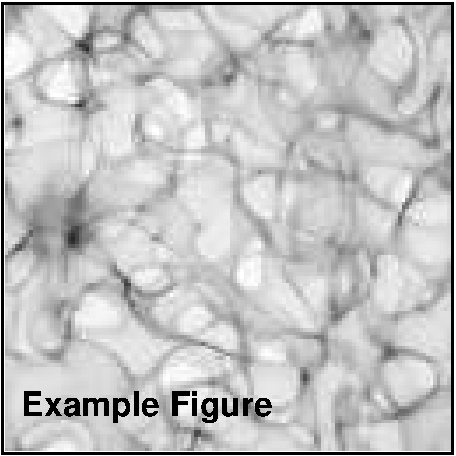
\includegraphics[width=\columnwidth]{example-fig}
  \caption{Example of a simple single-column figure.}
  \label{fig:simple}
\end{figure}

\begin{figure}[!t]
  
\includegraphics[width=0.56\columnwidth]{example-badfig}
  \hfill\parbox[b]{0.4\columnwidth}{\Large\textbf{Bad Bitmap Figure!}}
  \caption{How not to do a figure. This may not look so bad on the
    screen but try printing it out and you'll see what I mean.}
  \label{fig:bad}
\end{figure}

\begin{figure}[!t]\centering
  \vspace{0pt}
  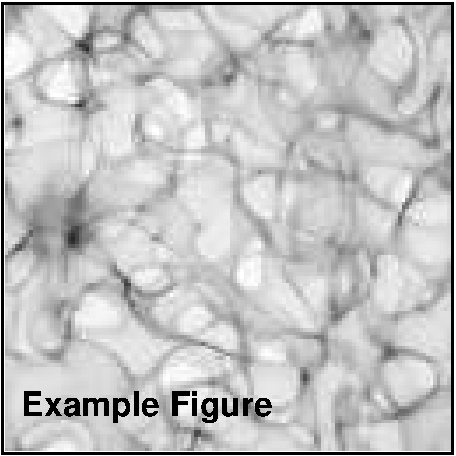
\includegraphics[angle=-90,width=0.8\columnwidth]{example-fig}
  \caption{Example of a rotated figure using the \texttt{angle}
    keyword to \CS{includegraphics}. Note that in the general case of
    a non-square figure, \texttt{angle=} should come before
    \texttt{width=} to avoid confusion. In this example the figure has
    also been reduced to 80\% of the column width and is centered by
    means of the \CS{centering} command. You should not use the
    \texttt{center} environment for this since it introduces unwanted
    vertical space.}
  \label{fig:rotate}
\end{figure}


\begin{figure}[!t]
  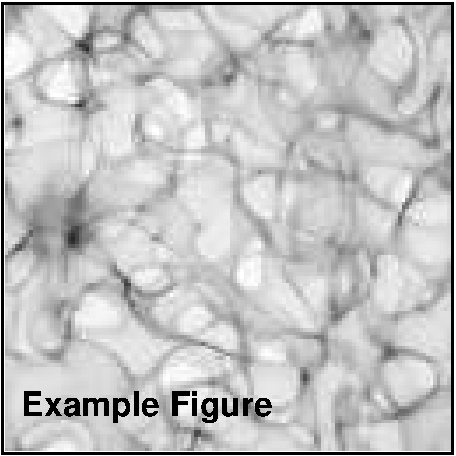
\includegraphics[bb=8 13 135 35,clip,width=\columnwidth]{example-fig}
  \caption{Example of a cropped figure using the \texttt{bb} and
    \texttt{clip} keywords. The syntax is ``\texttt{bb =} $x_0$ $y_0$
    $x_1$ $y_1$'' where $(x_0,y_0)$ and $(x_1,y_1)$ are the coordinates
    (in points) of the bottom-left and upper-right corner,
    respectively. Note that the EPS file used for this figure is the
    same as in the other examples.}
  \label{fig:crop}
\end{figure}

Figure~\ref{fig:simple} shows the simplest possible example of how to
include an EPS graphic file in a single-column figure. In order to
produce the highest-quality results and the smallest-possible EPS file
sizes, it is important to make sure you are using a vector format for
the text and line-art parts of the graphic. Failure to do so tends to
result in disasters like that shown in Figure~\ref{fig:bad}. Either
that, or, in an effort to produce acceptable quality lines and text
from a raster-format EPS file, you end up with the file being many
megabytes in size. A common cause of problems is the use programs such
as xv of ImageMagick. Once a postscript file has been read in by one
of these programs and then saved again (even if saved as postscript),
it has been irreversibly converted into a raster format, usually with
drastic concomitant loss of quality.

Sometimes your figure will come out sideways when you try to include
it. In this case you should use the \texttt{angle} keyword to
\CS{includegraphics}, as shown in Figure~\ref{fig:rotate}. 

On other occasions, you only want to include a certain portion of the
EPS graphic. This can be achieved by means of the \texttt{bbox}
keyword, which allows you to manually specify the graphic's bounding
box, as illustrated in Figure~\ref{fig:crop}. You will also want to
use the \texttt{clip} keyword to prevent the unwanted parts of the
figure from being displayed. This technique is also useful in cases
where the bounding box specified in the EPS file is not ``tight''
around the graphic. The easiest way to find the bounding box you want
is to load the EPS file in gv or a similar program. Then, when you
move the mouse cursor over the figure, the coordinates (in points) of
the current cursor position should be shown in a little window at the
top-left. Thus, it is straightforward to find the coordinates of the
bottom-left and top-right corners of the desired rectangular region.

% Programs commonly used for generating postscript graphics do not
% generally make it easy to do complicated text formatting on the labels
% you put on the graph (e.g., greek letters, math equations).
% Thankfully, by means of the optional \texttt{psfrag} package, you can
% get \LaTeX{} to do this formatting for you. Put
% \CS{usepackage\{psfrag\}} in your preamble, then use commands of the
% form
% \CS{psfrag}\{\textsc{label}\}\discretionary{}{}{}\{\textsc{replacement}\}
% inside your \texttt{figure} environment but before the
% \CS{includegraphics} command, where \textsc{label} is the text in the
% EPS file and \textsc{replacement} is arbitrary \LaTeX{} mark-up that
% you wish to replace it with. An example is shown in
% Figure~\ref{fig:psfrag}. A minor disadvantage of this approach is that
% the results are only visible in the postscript output of dvips, not in
% the DVI file when viewed with xdvi.

% \begin{figure}[t!]
%   \psfrag{Example Figure}{\colorbox{white}{Swirly stuff:
%       $\int_\alpha^\beta \mathcal{F}_\nu \, d\nu$}}
%   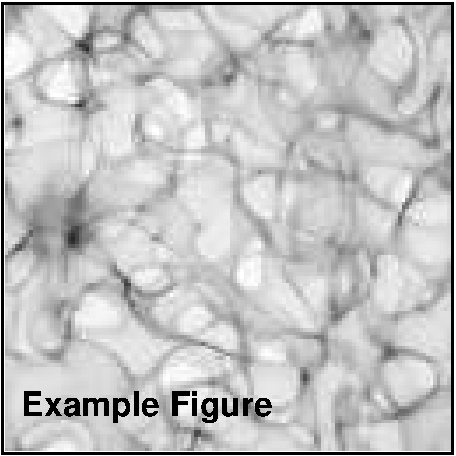
\includegraphics[width=\columnwidth]{example-fig}
%   \caption{Example of how to use the optional package \texttt{psfrag}
%     to perform replacement of strings in your EPS graphic by arbitrary
%     \LaTeX{} commands. Note that xdvi will not display this
%     correctly but the postscript output from dvips will be fine.  }
%   \label{fig:psfrag}
% \end{figure}

\begin{table}[!t]\centering
  \setlength{\tabnotewidth}{0.5\columnwidth}
  \tablecols{3}
  % Stretch the space between table columns 
  \setlength{\tabcolsep}{2.8\tabcolsep}
  \caption{A Simple Table (\lowercase{$x=1.0$})\tabnotemark{a}} \label{tab:ion_ab}
 \begin{tabular}{lrr}
    \toprule
    Ion & \multicolumn{1}{c}{NGC~5461} & \multicolumn{1}{c}{NGC~5471} \\
    \midrule
    O$^0$    & $7.08\pm0.20$ & $6.63\pm0.20$\\
    O$^+$    & $8.08\pm0.14$ & $7.32\pm0.14$\\
    O$^{++}$ & $8.32\pm0.07$ & $8.02\pm0.07$\\
    N$^+$    & $7.04\pm0.12$ & $6.01\pm0.13$\\
    Ne$^{++}$ & $7.59\pm0.11$ & $7.32\pm0.10$\\
    S$^+$    & $6.02\pm0.19$ & $5.47\pm0.20$\\
    S$^{++}$ & $7.00\pm0.10$ & $6.45\pm0.10$\\
    Cl$^{++}$ & $4.93\pm0.16$ & $4.20\pm0.16$\\
    Ar$^{++}$ & $6.15\pm0.12$ & $5.55\pm0.14$\\
    Ar$^{3+}$ &\multicolumn{1}{c}{\nodata} & $5.07\pm0.10$\\
    \bottomrule
    \tabnotetext{a}{Note the use of \CS{lowercase} to prevent the $x$
        from being converted to upper case.}
  \end{tabular}
\end{table}

Figure~\ref{fig:widefig1} shows a double-column figure containing two
EPS graphics and Figure~\ref{fig:widefig2} is a more complicated
example of the same. 

\begin{figure*}[!t]
  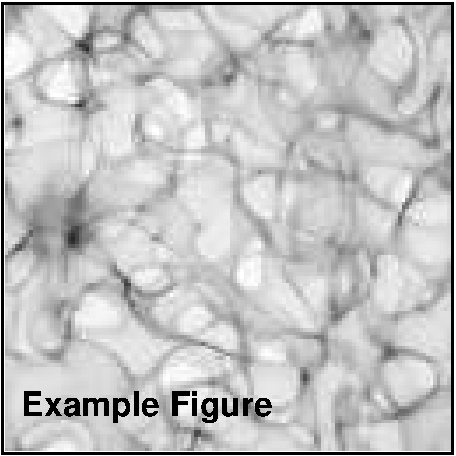
\includegraphics[width=0.45\linewidth,height=3cm]{example-fig}%
  \hfill
  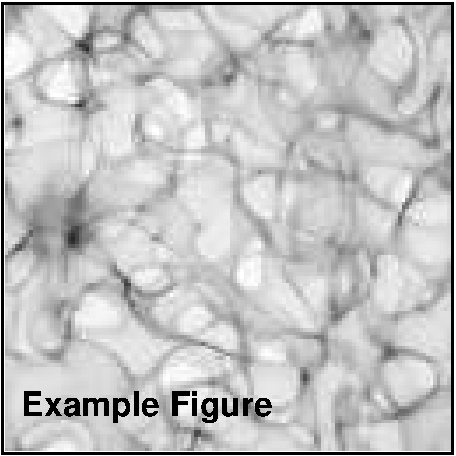
\includegraphics[width=0.45\linewidth,height=3cm]{example-fig}
  \caption{Simple example of a wide figure that spans both
    columns and includes two EPS files. The individual EPS graphic
    widths and spacing between them are set to be the same as that of
    the columns of text (\CS{columnwidth} and \CS{columnsep})
    respectively. Note the use of \texttt{\%} to suppress unwanted
    spaces. Alternatively, you may want a single EPS graphic to span
    the entire width, in which case you would put
    \texttt{width=\CS{textwidth}} instead. In this example, both the
    \texttt{width} and \texttt{height} keywords are used, forcing the
    scaling to be anisotropic. You will never normally want to do
    this.}
  \label{fig:widefig1}
\end{figure*}

\begin{figure*}[!t]
  \newlength\thisfigwidth
  \setlength\thisfigwidth{0.5\linewidth}
  \addtolength\thisfigwidth{-0.5cm}
  \begin{tabular}{ll}
    \textbf{a} & \textbf{b} \\
    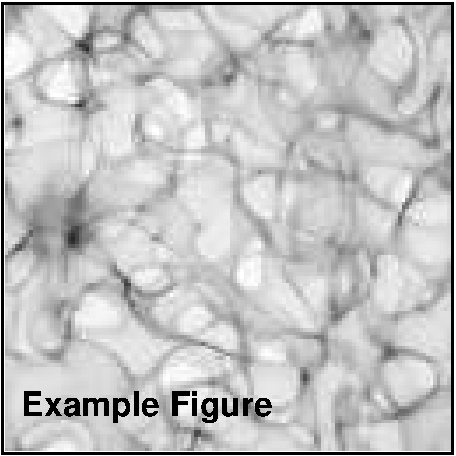
\includegraphics[width=\thisfigwidth,height=3cm]{example-fig}
    & 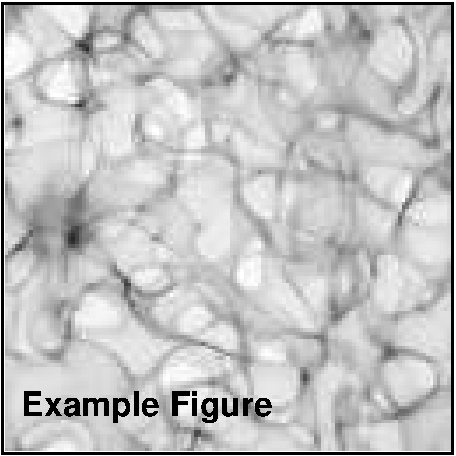
\includegraphics[width=\thisfigwidth,height=3cm]{example-fig}
  \end{tabular}
  \caption{A more complicated example of a multipart figure, using
    \LaTeX{} itself to put the \textbf{a} and \textbf{b} labels
    on. (\textit{a}) Multipart figures are captioned like this.
    (\textit{b}) The second part of the figure.  Note that the
    \texttt{tabular} environment is an easy way to arrange the
    subfigures and their labels.  }
  \label{fig:widefig2}
\end{figure*}


\paragraph{Color Graphics}

Color plates greatly increases the printing costs and so are best
avoided. On the other hand, including color figures in the online
version costs nothing. The best solution is for the author to provide
alternative grayscale versions of any color images, which can then be
used in the printed version. Otherwise, the way your beautiful color
picture gets converted to black-and-white will be entirely at the
mercy of the editors and printers. Remember, too, that grayscale
images generally look better on a negative scale.

\section{How To Do Tables}
\label{sec:how-do-tables}

An example of a simple table is given in Table~\ref{tab:ion_ab}. Some
points to note are:
\begin{enumerate}
\item We use the \texttt{booktabs} package (loaded automatically),
  which gives improved vertical layout with respect to the standard
  \LaTeX{} version. As a user, the only impact of this is that you
  must use \CS{toprule}, \CS{midrule}, and \CS{bottomrule} instead of
  \CS{hline} to give the horizontal rules. Vertical rules should never
  be used. 
\item Footnotes to the table can be entered using a
  \CS{tabnotemark}, \CS{tabnotetext} pair. Note that \CS{tabnotetext}
  occurs inside the \texttt{tabular} environment and that for it to
  work properly you must use the \CS{tablecols} command to specify the
  number of columns in the table and set the length \CS{tabnotewidth}
  to a sensible value.
\item The intercolumn spacing can be adjusted by setting the length
  \CS{tabcolsep}. Things usually look best when this is set so that
  the table fills the entire width of a text column as closely as
  possible. 
\item Missing data is indicated by the \CS{nodata} command, as in
  AAS\TeX. 
\end{enumerate}


Table~\ref{tab:ioniz_av_landscape} is a somewhat more complicated
example. Some features of this example are:
\begin{enumerate}
\item The use of \CS{cmidrule} for partial horizontal rules. 
\item Somewhat elaborate adjustments to the horizontal spacing so as
  to visually tie together subgroups of the columns. Two different
  mechanisms are used to achieve this. That of putting in an empty
  ``ghost'' column is probably the easiest to manage. The other is to
  use the \verb+@+ specifier with a user-defined horizontal space.
\item The table is wider than will fit in the normal text width. To
  remedy this, we wrap the table inside the \texttt{landscape}
  environment, which rotates the entire page by 90 degrees.  A
  disadvantage of this approach is that the article text cannot flow
  around the table, which is forced to appear on its own page.  This
  requires that either the \texttt{lscape} or \texttt{pdflscape}
  package must be loaded in the preamble. 
\end{enumerate}

If your table will not fit on one page (even when rotated), then you
can use the \texttt{longtable} package. I can provide an example of
this on request.

\begin{landscape}
  \begin{table}
    \newcommand{\DS}{\hspace{6\tabcolsep}} %% Expanded Space between
    %% some cols
    \caption{A more involved table that is rotated to fit better on
      the page\tabnotemark{a}}
    \label{tab:ioniz_av_landscape}
    \setlength{\tabnotewidth}{0.65\linewidth}
    \setlength{\tabcolsep}{1.2\tabcolsep}
    \tablecols{10}
    \centering
    \begin{tabular}{l @{\DS} cccc l cccc}
      \toprule
      & \multicolumn{9}{c}{Ionization Stage}\\
      \cmidrule{3-9}
      & \multicolumn{4}{c}{Log (Radial Average)}
      &&\multicolumn{4}{c}{Log (Volume Average)}\\
      \cmidrule(r){2-5}\cmidrule(l){7-10}
      Element& I & II & III & IV && I & II & III & IV \\
      \midrule
      Hydrogen & $-2.738$ & $-0.001$ &  \nodata &  \nodata  && $-1.610$ &
      $-0.011$ &  \nodata  &  \nodata  \\ 
      Helium   & $-1.661$ & $-0.009$ &  \nodata &  \nodata  && $-0.567$ &
      $-0.137$ &  \nodata  &  \nodata  \\ 
      Nitrogen & $-3.045$ & $-0.836$ & $-0.069$ & $-3.605$  && $-1.785$ &
      $-0.270$ & $-0.351$  & $-4.288$  \\ 
      Oxygen   & $-2.822$ & $-0.452$ & $-0.191$ &  \nodata  && $-1.584$ &
      $-0.150$ & $-0.574$  &  \nodata  \\ 
      Neon     & $-2.842$ & $-0.169$ & $-0.494$ &  \nodata  && $-1.815$ &
      $-0.058$ & $-0.960$  &  \nodata  \\ 
      Sulfur   & $-5.322$ & $-1.276$ & $-0.042$ & $-1.420$  && $-4.247$ &
      $-0.597$ & $-0.132$  & $-2.069$  \\ 
      Chlorine & $-4.716$ & $-1.093$ & $-0.041$ & $-2.037$  && $-3.644$ &
      $-0.477$ & $-0.177$  & $-2.689$  \\ 
      Argon    & $-3.585$ & $-1.382$ & $-0.023$ & $-1.996$  && $-2.283$ &
      $-0.490$ & $-0.175$  & $-2.657$  \\ 
      \bottomrule
      \tabnotetext{a}{\small The original of this and the
        previous table come  
      from Luridiana et~al.\@ (2002) RevMexAA 38, 97.}
    \end{tabular}
  \end{table}
\end{landscape}


\section{How To Do References}
\label{sec:refs}

The style of the reference list follows that of the ApJ, AJ, etc. That
is:
\begin{compactitem}
\item Comma after each surname, space between initials (unlike A\&A).
\item No comma before year.
\item Commas everywhere else. 
\item If there are more then 6 authors you should use et~al.
\end{compactitem}
An almost bulletproof way of getting your reference list right is to
grab them from ADS (select ``AASTEX reference style''). The
\texttt{rmaa} macros recognize all the AAS journal abbreviation
commands. 

In the text, references should be cited as follows: 
\begin{Example}
  \dots it has been found (Garc\'\i{}a 1990; L\'opez 2000a,b) that \dots
  following Bloggs (1990) \dots is not true (despite what
  Rodr\'\i{}guez 1759 maintains) \dots
\end{Example}
Note the use of semicolons between consecutive references and the lack
of comma between author and date. In order to save effort and reduce
errors, it is preferable to use commands from the \texttt{natbib}
package to automate the references in the text, as in the following
example:
\begin{Example}
  \dots it has been found \citep{2005astro.ph.11035A,
    1991ApJ...374..580B, 2005MNRAS.358..291D} that \dots following
  \citet{1996ApJ...469..171G} \dots is not true (despite what
  \citealp{1939ApJ....89..526S} maintains) \dots
\end{Example}
See \texttt{authorguide.pdf} for more examples and explanation.  For
the reference keys, one can use the ADS bibliographic code, which is
the default for references obtained from ADS. Alternatively, if these
prove too hard to remember\footnote{There is no need to remember the
  keys if you use an editor that understands \LaTeX{} references, such
  as RefTeX mode in emacs.}, any mnemonic string may be used.

It is also possible to automate the generation of the reference list
itself using BibTeX, but support for this in the macros is still
experimental. For further details, see \texttt{authorguide.pdf}.

\acknowledgments Acknowledgements of grants received, assistance from
colleagues, and helpful referees follow the \CS{acknowledgments}
command, which simply adds a bit of vertical space.

\begin{appendix}
  \section{How to make an appendix}
  Appendices come before the references (unlike in some other
  journals). Each appendix is introduced by a \CS{section} command,
  which should be placed inside an \texttt{appendices} environment (or
  an \texttt{appendix} environment if there is only one).
\end{appendix}



\begin{thebibliography}
\bibitem[Arthur \& Hoare(2006)]{2005astro.ph.11035A} Arthur, S.~J., \&
Hoare, M.~G.\ 2006, \apj, in press (astro-ph/0511035)
\bibitem[Baldwin et al.(1991)]{1991ApJ...374..580B} Baldwin, J.~A., 
Ferland, G.~J., Martin, P.~G., Corbin, M.~R., Cota, S.~A., Peterson, B.~M., 
\& Slettebak, A.\ 1991, \apj, 374, 580 
\bibitem[Bedijn \& Tenorio-Tagle(1981)]{1981A&A....98...85B} Bedijn, P.~J., 
\& Tenorio-Tagle, G.\ 1981, \aap, 98, 85 
\bibitem[Bodenheimer et al.(1979)]{1979ApJ...233...85B} Bodenheimer, P., 
Tenorio-Tagle, G., \& Yorke, H.~W.\ 1979, \apj, 233, 85 
\bibitem[Carlqvist et al.(2003)]{2003A&A...403..399C} Carlqvist, P., Gahm, 
G.~F., \& Kristen, H.\ 2003, \aap, 403, 399 
\bibitem[Dale et al.(2005)]{2005MNRAS.358..291D} Dale, J.~E., Bonnell, 
I.~A., Clarke, C.~J., \& Bate, M.~R.\ 2005, \mnras, 358, 291 
\bibitem[Elmegreen \& Scalo(2004)]{2004ARA&A..42..211E} Elmegreen,
B.~G., \& Scalo, J.\ 2004, \araa, 42, 211 
\bibitem[Eulderink \& Mellema(1995)]{1995A&AS..110..587E} Eulderink, F., \& 
Mellema, G.\ 1995, \aaps, 110, 587 
\bibitem[Ferland(2000)]{2000RMxAC...9..153F} Ferland, G.~J.\ 2000, Revista 
Mexicana de Astronom\'\i{}a y Astrof\'\i{}sica Conference Series, 9, 153 
\bibitem[Franco et al.(1989)]{1989RMxAA..18...65F} Franco, J., 
Tenorio-Tagle, G., \& Bodenheimer, P.\ 1989, Revista Mexicana de
Astronom\'\i{}a y Astrof\'\i{}sica, 18, 65 
\bibitem[Franco et al.(1990)]{1990ApJ...349..126F} Franco, J., 
Tenorio-Tagle, G., \& Bodenheimer, P.\ 1990, \apj, 349, 126 
\bibitem[Garc\'\i a-Segura \& Franco(1996)]{1996ApJ...469..171G}
  Garc\'\i a-Segura, G., \& Franco, J.\ 1996, \apj, 469, 171
\bibitem[Giuliani(1979)]{1979ApJ...233..280G} Giuliani, J.~L.\ 1979,
\apj, 233, 280 
\bibitem[Henney(2006)]{2006-FS-Will} Henney, W.~J.\ 2006, In:
  \textit{Diffuse Matter from Star Forming Regions to Active Galaxies:
    A Volume Honouring John Dyson.} Eds.\ T.~W. Harquist,
  J.~M. Pittard, \& S.~A.~E.~G. Falle. (Dordrecht: Springer), in press
  (astro-ph/0602626)
 \bibitem[Henney et al.(2005a)]{2005ApJ...627..813H} Henney, W.~J.,
Arthur, S.~J., \& Garc{\'{\i}}a-D{\'{\i}}az, M.~T.\ 2005, \apj, 627, 813 
\bibitem[Henney et al.(2005b)]{2005ApJ...621..328H} Henney, W.~J., Arthur, 
S.~J., Williams, R.~J.~R., \& Ferland, G.~J.\ 2005, \apj, 621, 328 
\bibitem[Hester et al.(1996)]{1996AJ....111.2349H} Hester, J.~J., et
al.\ 1996, \aj, 111, 2349 
\bibitem[Iliev et al.(2006a)]{reion_sim} Iliev, I. T., Mellema, G.,
  Pen, U.-L., Merz, H., Shapiro, P. R., \& Alvarez, M.~A.  2006a,
  MNRAS, submitted (astro-ph/0512187)
\bibitem[Iliev et al.(2006b)]{2006astro.ph..3199I} Iliev, I.~T., et
  al.\ 2006b, \mnras, submitted (astro-ph/0603199)
\bibitem[Iliev et al.(2006c)]{2006CodeComparison} Iliev, I.~T., et
  al.\ 2006c, in preparation (Cosmological Radiative Transfer Code Comparison  
  \url{http://www.mpa-garching.mpg.de/tsu3/})
\bibitem[Kahn(1954)]{1954BAN....12..187K} Kahn, F.~D.\ 1954, \bain, 12, 187 
\bibitem[Klessen et al.(2000)]{2000ApJ...535..887K} Klessen, R.~S.,
  Heitsch, F., \& Mac Low, M.-M.\ 2000, \apj, 535, 887
\bibitem[Lada \& Lada(2003)]{2003ARA&A..41...57L} Lada, C.~J., \&
Lada, E.~A.\ 2003, \araa, 41, 57 
\bibitem[Larson(1981)]{1981MNRAS.194..809L} Larson, R.~B.\ 1981,
\mnras, 194, 809 
\bibitem[Li et al.(2004)]{2004ApJ...610..339L} Li, Y., Mac Low, M.-M.,
\& Abel, T.\ 2004, \apj, 610, 339 
\bibitem[Mellema et al.(2006)]{2005astro.ph..8416M} Mellema, G.,
  Iliev, I.~T., Alvarez, M.~A., \& Shapiro, P.~R.\ 2006, New
  Astronomy, 11, 374 (astro-ph/0508416)
\bibitem[Moffat et al.(2002)]{2002ApJ...573..191M} Moffat, A.~F.~J., et 
al.\ 2002, \apj, 573, 191 
\bibitem[O'Dell(2001)]{2001ARA&A..39...99O} O'Dell, C.~R.\ 2001, \araa, 39, 
99 
\bibitem[O'Dell et al.(2003)]{2003AJ....125.2590O} O'Dell, C.~R., Peimbert, 
M., \& Peimbert, A.\ 2003, \aj, 125, 2590 
 \bibitem[O'Dell \& Yusef-Zadeh(2000)]{2000AJ....120..382O} O'Dell, C.~R., 
\& Yusef-Zadeh, F.\ 2000, \aj, 120, 382 
\bibitem[Panagia(1973)]{1973AJ.....78..929P} Panagia, N.\ 1973, \aj,
78, 929 
\bibitem[Pottasch(1956)]{1956BAN....13...77P} Pottasch, S.~R.\ 1956, \bain, 
13, 77 
\bibitem[Raga et al.(1999)]{1999RMxAA..35..123R} Raga, A.~C., Mellema, G., 
Arthur, S.~J., Binette, L., Ferruit, P., \& Steffen, W.\ 1999, Revista 
Mexicana de Astronom\'\i{}a y Astrof\'\i{}sica, 35, 123
\bibitem[Redman et al.(1998)]{1998A&A...331.1099R} Redman, M.~P., Williams, 
R.~J.~R., Dyson, J.~E., Hartquist, T.~W., \& Fernandez, B.~R.\ 1998, \aap, 
331, 1099 
\bibitem[Rho et al.(2005)]{2005sfet.confE..15R} Rho, J., Reach, W.~T., 
Lefloch, B., \& Fazio, G.\ 2005, In: Star Formation in the Era of Three Great 
Observatories, see
\url{http://www.spitzer.caltech.edu/Media/releases/ssc2005-02/ssc2005-02a.shtml}
\bibitem[Ryutov et al.(2005)]{2005Ap&SS.298..183R} Ryutov, D.~D., Kane, 
J.~O., Mizuta, A., Pound, M.~W., \& Remington, B.~A.\ 2005, \apss, 298, 183 
\bibitem[Scowen et al.(1998)]{1998AJ....116..163S} Scowen, P.~A., et al.\ 
1998, \aj, 116, 163 
\bibitem[Shu et al.(2002)]{2002ApJ...580..969S} Shu, F.~H., Lizano, S., 
Galli, D., Cant{\'o}, J., \& Laughlin, G.\ 2002, \apj, 580, 969 
\bibitem[Spitzer(1968)]{1968dms..book.....S} Spitzer, L.\ 1968,
  Diffuse Matter in Space, New York: Interscience
\adjustfinalcols
\bibitem[Str{\"o}mgren(1939)]{1939ApJ....89..526S} Str{\"o}mgren, B.\ 1939, 
\apj, 89, 526 
\bibitem[Sutherland et al.(2003)]{2003ApJS..147..187S} Sutherland,
R.~S., Bisset, D.~K., \& Bicknell, G.~V.\ 2003, \apjs, 147, 187 
\bibitem[Tenorio-Tagle(1979)]{1979A&A....71...59T} Tenorio-Tagle, G.\ 1979, 
\aap, 71, 59 
\bibitem[Tenorio-Tagle et al.(2006)]{2006astro.ph..1631T}
  Tenorio-Tagle, G., Mu\~noz-Tu\~n\'on, C., P\'erez, E., Silich, S., \&
  Telles, E.\ 2006, \apj, in press (astro-ph/0601631)
\bibitem[V\'azquez-Semadeni et al.(2000)]{2000prpl.conf....3V} 
V\'azquez-Semadeni, E., Ostriker, E.~C., Passot, T., Gammie, C.~F., \&
Stone, J.~M.\ 2000, Protostars and Planets IV, 3 
\bibitem[V{\'a}zquez-Semadeni et al.(2003)]{2003ApJ...585L.131V} 
V{\'a}zquez-Semadeni, E., Ballesteros-Paredes, J., \& Klessen, R.~S.\
2003, \apjl, 585, L131 
\bibitem[V{\'a}zquez-Semadeni et al.(2005)]{2005ApJ...630L..49V} 
V{\'a}zquez-Semadeni, E., Kim, J., \& Ballesteros-Paredes, J.\ 2005,
\apjl, 630, L49 
\bibitem[V{\'a}zquez-Semadeni et al.(2005)]{2005ApJ...618..344V} 
V{\'a}zquez-Semadeni, E., Kim, J., Shadmehri, M., \&
Ballesteros-Paredes, J.\ 2005, \apj, 618, 344 
\bibitem[Williams(1999)]{1999MNRAS.310..789W} Williams, R.~J.~R.\
1999, \mnras, 310, 789 
\bibitem[Williams(2006)]{2006-FS-Robin} Williams, R.~J.~R.\ 2006, In:
  \textit{Diffuse Matter from Star Forming Regions to Active
    Galaxies: A Volume Honouring John Dyson.} Eds.\ T.~W. Harquist,
  J.~M. Pittard, \& S.~A.~E.~G. Falle. (Dordrecht: Springer), in press
\bibitem[Williams \& Dyson(2001)]{2001MNRAS.325..293W} Williams, R.~J.~R., 
\& Dyson, J.~E.\ 2001, \mnras, 325, 293 
\bibitem[Williams et al.(2000)]{2000MNRAS.314..315W} Williams, R.~J.~R., 
Dyson, J.~E., \& Hartquist, T.~W.\ 2000, \mnras, 314, 315 
\bibitem[Wood \& Churchwell(1989)]{1989ApJS...69..831W} Wood, D.~O.~S., \& 
Churchwell, E.\ 1989, \apjs, 69, 831 
\end{thebibliography}

\end{document}

%%% Local Variables:
%%% mode: latex
%%% TeX-master: t
%%% End:
